% Options for packages loaded elsewhere
\PassOptionsToPackage{unicode}{hyperref}
\PassOptionsToPackage{hyphens}{url}
\PassOptionsToPackage{dvipsnames,svgnames,x11names}{xcolor}
%
\documentclass[
  letterpaper,
  DIV=11,
  numbers=noendperiod]{scrreprt}

\usepackage{amsmath,amssymb}
\usepackage{lmodern}
\usepackage{iftex}
\ifPDFTeX
  \usepackage[T1]{fontenc}
  \usepackage[utf8]{inputenc}
  \usepackage{textcomp} % provide euro and other symbols
\else % if luatex or xetex
  \usepackage{unicode-math}
  \defaultfontfeatures{Scale=MatchLowercase}
  \defaultfontfeatures[\rmfamily]{Ligatures=TeX,Scale=1}
\fi
% Use upquote if available, for straight quotes in verbatim environments
\IfFileExists{upquote.sty}{\usepackage{upquote}}{}
\IfFileExists{microtype.sty}{% use microtype if available
  \usepackage[]{microtype}
  \UseMicrotypeSet[protrusion]{basicmath} % disable protrusion for tt fonts
}{}
\makeatletter
\@ifundefined{KOMAClassName}{% if non-KOMA class
  \IfFileExists{parskip.sty}{%
    \usepackage{parskip}
  }{% else
    \setlength{\parindent}{0pt}
    \setlength{\parskip}{6pt plus 2pt minus 1pt}}
}{% if KOMA class
  \KOMAoptions{parskip=half}}
\makeatother
\usepackage{xcolor}
\setlength{\emergencystretch}{3em} % prevent overfull lines
\setcounter{secnumdepth}{-\maxdimen} % remove section numbering
% Make \paragraph and \subparagraph free-standing
\ifx\paragraph\undefined\else
  \let\oldparagraph\paragraph
  \renewcommand{\paragraph}[1]{\oldparagraph{#1}\mbox{}}
\fi
\ifx\subparagraph\undefined\else
  \let\oldsubparagraph\subparagraph
  \renewcommand{\subparagraph}[1]{\oldsubparagraph{#1}\mbox{}}
\fi

\usepackage{color}
\usepackage{fancyvrb}
\newcommand{\VerbBar}{|}
\newcommand{\VERB}{\Verb[commandchars=\\\{\}]}
\DefineVerbatimEnvironment{Highlighting}{Verbatim}{commandchars=\\\{\}}
% Add ',fontsize=\small' for more characters per line
\usepackage{framed}
\definecolor{shadecolor}{RGB}{241,243,245}
\newenvironment{Shaded}{\begin{snugshade}}{\end{snugshade}}
\newcommand{\AlertTok}[1]{\textcolor[rgb]{0.68,0.00,0.00}{#1}}
\newcommand{\AnnotationTok}[1]{\textcolor[rgb]{0.37,0.37,0.37}{#1}}
\newcommand{\AttributeTok}[1]{\textcolor[rgb]{0.40,0.45,0.13}{#1}}
\newcommand{\BaseNTok}[1]{\textcolor[rgb]{0.68,0.00,0.00}{#1}}
\newcommand{\BuiltInTok}[1]{\textcolor[rgb]{0.00,0.23,0.31}{#1}}
\newcommand{\CharTok}[1]{\textcolor[rgb]{0.13,0.47,0.30}{#1}}
\newcommand{\CommentTok}[1]{\textcolor[rgb]{0.37,0.37,0.37}{#1}}
\newcommand{\CommentVarTok}[1]{\textcolor[rgb]{0.37,0.37,0.37}{\textit{#1}}}
\newcommand{\ConstantTok}[1]{\textcolor[rgb]{0.56,0.35,0.01}{#1}}
\newcommand{\ControlFlowTok}[1]{\textcolor[rgb]{0.00,0.23,0.31}{#1}}
\newcommand{\DataTypeTok}[1]{\textcolor[rgb]{0.68,0.00,0.00}{#1}}
\newcommand{\DecValTok}[1]{\textcolor[rgb]{0.68,0.00,0.00}{#1}}
\newcommand{\DocumentationTok}[1]{\textcolor[rgb]{0.37,0.37,0.37}{\textit{#1}}}
\newcommand{\ErrorTok}[1]{\textcolor[rgb]{0.68,0.00,0.00}{#1}}
\newcommand{\ExtensionTok}[1]{\textcolor[rgb]{0.00,0.23,0.31}{#1}}
\newcommand{\FloatTok}[1]{\textcolor[rgb]{0.68,0.00,0.00}{#1}}
\newcommand{\FunctionTok}[1]{\textcolor[rgb]{0.28,0.35,0.67}{#1}}
\newcommand{\ImportTok}[1]{\textcolor[rgb]{0.00,0.46,0.62}{#1}}
\newcommand{\InformationTok}[1]{\textcolor[rgb]{0.37,0.37,0.37}{#1}}
\newcommand{\KeywordTok}[1]{\textcolor[rgb]{0.00,0.23,0.31}{#1}}
\newcommand{\NormalTok}[1]{\textcolor[rgb]{0.00,0.23,0.31}{#1}}
\newcommand{\OperatorTok}[1]{\textcolor[rgb]{0.37,0.37,0.37}{#1}}
\newcommand{\OtherTok}[1]{\textcolor[rgb]{0.00,0.23,0.31}{#1}}
\newcommand{\PreprocessorTok}[1]{\textcolor[rgb]{0.68,0.00,0.00}{#1}}
\newcommand{\RegionMarkerTok}[1]{\textcolor[rgb]{0.00,0.23,0.31}{#1}}
\newcommand{\SpecialCharTok}[1]{\textcolor[rgb]{0.37,0.37,0.37}{#1}}
\newcommand{\SpecialStringTok}[1]{\textcolor[rgb]{0.13,0.47,0.30}{#1}}
\newcommand{\StringTok}[1]{\textcolor[rgb]{0.13,0.47,0.30}{#1}}
\newcommand{\VariableTok}[1]{\textcolor[rgb]{0.07,0.07,0.07}{#1}}
\newcommand{\VerbatimStringTok}[1]{\textcolor[rgb]{0.13,0.47,0.30}{#1}}
\newcommand{\WarningTok}[1]{\textcolor[rgb]{0.37,0.37,0.37}{\textit{#1}}}

\providecommand{\tightlist}{%
  \setlength{\itemsep}{0pt}\setlength{\parskip}{0pt}}\usepackage{longtable,booktabs,array}
\usepackage{calc} % for calculating minipage widths
% Correct order of tables after \paragraph or \subparagraph
\usepackage{etoolbox}
\makeatletter
\patchcmd\longtable{\par}{\if@noskipsec\mbox{}\fi\par}{}{}
\makeatother
% Allow footnotes in longtable head/foot
\IfFileExists{footnotehyper.sty}{\usepackage{footnotehyper}}{\usepackage{footnote}}
\makesavenoteenv{longtable}
\usepackage{graphicx}
\makeatletter
\def\maxwidth{\ifdim\Gin@nat@width>\linewidth\linewidth\else\Gin@nat@width\fi}
\def\maxheight{\ifdim\Gin@nat@height>\textheight\textheight\else\Gin@nat@height\fi}
\makeatother
% Scale images if necessary, so that they will not overflow the page
% margins by default, and it is still possible to overwrite the defaults
% using explicit options in \includegraphics[width, height, ...]{}
\setkeys{Gin}{width=\maxwidth,height=\maxheight,keepaspectratio}
% Set default figure placement to htbp
\makeatletter
\def\fps@figure{htbp}
\makeatother

\KOMAoption{captions}{tableheading}
\makeatletter
\makeatother
\makeatletter
\makeatother
\makeatletter
\@ifpackageloaded{caption}{}{\usepackage{caption}}
\AtBeginDocument{%
\ifdefined\contentsname
  \renewcommand*\contentsname{Table of contents}
\else
  \newcommand\contentsname{Table of contents}
\fi
\ifdefined\listfigurename
  \renewcommand*\listfigurename{List of Figures}
\else
  \newcommand\listfigurename{List of Figures}
\fi
\ifdefined\listtablename
  \renewcommand*\listtablename{List of Tables}
\else
  \newcommand\listtablename{List of Tables}
\fi
\ifdefined\figurename
  \renewcommand*\figurename{Figure}
\else
  \newcommand\figurename{Figure}
\fi
\ifdefined\tablename
  \renewcommand*\tablename{Table}
\else
  \newcommand\tablename{Table}
\fi
}
\@ifpackageloaded{float}{}{\usepackage{float}}
\floatstyle{ruled}
\@ifundefined{c@chapter}{\newfloat{codelisting}{h}{lop}}{\newfloat{codelisting}{h}{lop}[chapter]}
\floatname{codelisting}{Listing}
\newcommand*\listoflistings{\listof{codelisting}{List of Listings}}
\makeatother
\makeatletter
\@ifpackageloaded{caption}{}{\usepackage{caption}}
\@ifpackageloaded{subcaption}{}{\usepackage{subcaption}}
\makeatother
\makeatletter
\@ifpackageloaded{tcolorbox}{}{\usepackage[many]{tcolorbox}}
\makeatother
\makeatletter
\@ifundefined{shadecolor}{\definecolor{shadecolor}{rgb}{.97, .97, .97}}
\makeatother
\makeatletter
\makeatother
\ifLuaTeX
  \usepackage{selnolig}  % disable illegal ligatures
\fi
\IfFileExists{bookmark.sty}{\usepackage{bookmark}}{\usepackage{hyperref}}
\IfFileExists{xurl.sty}{\usepackage{xurl}}{} % add URL line breaks if available
\urlstyle{same} % disable monospaced font for URLs
\hypersetup{
  pdftitle={My first R Markdown script},
  pdfauthor={Your name},
  colorlinks=true,
  linkcolor={blue},
  filecolor={Maroon},
  citecolor={Blue},
  urlcolor={Blue},
  pdfcreator={LaTeX via pandoc}}

\title{My first R Markdown script}
\author{Your name}
\date{11/22/24}

\begin{document}
\maketitle
\ifdefined\Shaded\renewenvironment{Shaded}{\begin{tcolorbox}[boxrule=0pt, breakable, borderline west={3pt}{0pt}{shadecolor}, sharp corners, frame hidden, enhanced, interior hidden]}{\end{tcolorbox}}\fi

\renewcommand*\contentsname{Table of contents}
{
\hypersetup{linkcolor=}
\setcounter{tocdepth}{3}
\tableofcontents
}
\hypertarget{prepare-to-work}{%
\chapter{1. Prepare to work}\label{prepare-to-work}}

\hypertarget{set-the-working-directory}{%
\section{1.1 Set the working
directory}\label{set-the-working-directory}}

Refer to Section 1.2 for this, Part 3.1.

\hypertarget{load-the-libraries}{%
\section{1.2 Load the libraries}\label{load-the-libraries}}

\begin{Shaded}
\begin{Highlighting}[]
\FunctionTok{library}\NormalTok{(dplyr)}
\end{Highlighting}
\end{Shaded}

\hypertarget{load-the-data}{%
\section{1.3 Load the data}\label{load-the-data}}

\begin{Shaded}
\begin{Highlighting}[]
\NormalTok{data }\OtherTok{\textless{}{-}} \FunctionTok{read.csv}\NormalTok{(}\StringTok{"\textasciitilde{}/Fake/GACTT\_RESULTS\_ANONYMIZED\_v2.csv"}\NormalTok{, }\AttributeTok{header=}\ConstantTok{TRUE}\NormalTok{)}
\end{Highlighting}
\end{Shaded}

\hypertarget{preliminary-observations-and-preparation-of-the-data}{%
\chapter{2. Preliminary observations and preparation of the
data}\label{preliminary-observations-and-preparation-of-the-data}}

\hypertarget{preliminary-descriptive-statistics}{%
\section{2.1 Preliminary descriptive
statistics}\label{preliminary-descriptive-statistics}}

\begin{Shaded}
\begin{Highlighting}[]
\DocumentationTok{\#\# head(data, 5) \#\# Code not run because too lengthy}
\DocumentationTok{\#\# str(data) \#\# Code not run because too lengthy}
\DocumentationTok{\#\# summary(data) \#\# Code not run because too lengthy}
\end{Highlighting}
\end{Shaded}

\hypertarget{transformation-of-the-data}{%
\section{2.2 Transformation of the
data}\label{transformation-of-the-data}}

\hypertarget{change-of-class}{%
\subsection{2.2.1 Change of class}\label{change-of-class}}

\begin{Shaded}
\begin{Highlighting}[]
\NormalTok{data}\SpecialCharTok{$}\NormalTok{What.is.your.age. }\OtherTok{\textless{}{-}} \FunctionTok{as.factor}\NormalTok{(data}\SpecialCharTok{$}\NormalTok{What.is.your.age.)}
\NormalTok{data}\SpecialCharTok{$}\NormalTok{How.many.cups.of.coffee.do.you.typically.drink.per.day. }\OtherTok{\textless{}{-}} \FunctionTok{as.factor}\NormalTok{(data}\SpecialCharTok{$}\NormalTok{How.many.cups.of.coffee.do.you.typically.drink.per.day.)}
\NormalTok{data}\SpecialCharTok{$}\NormalTok{Where.do.you.typically.drink.coffee. }\OtherTok{\textless{}{-}} \FunctionTok{as.factor}\NormalTok{(data}\SpecialCharTok{$}\NormalTok{Where.do.you.typically.drink.coffee.)}
\DocumentationTok{\#\# summary(data) \#\# Code not run because too lengthy}
\end{Highlighting}
\end{Shaded}

\begin{Shaded}
\begin{Highlighting}[]
\FunctionTok{levels}\NormalTok{(data}\SpecialCharTok{$}\NormalTok{What.is.your.age.)}
\end{Highlighting}
\end{Shaded}

\begin{verbatim}
[1] ""                "<18 years old"   ">65 years old"   "18-24 years old"
[5] "25-34 years old" "35-44 years old" "45-54 years old" "55-64 years old"
\end{verbatim}

\begin{Shaded}
\begin{Highlighting}[]
\FunctionTok{levels}\NormalTok{(data}\SpecialCharTok{$}\NormalTok{How.many.cups.of.coffee.do.you.typically.drink.per.day.)}
\end{Highlighting}
\end{Shaded}

\begin{verbatim}
[1] ""            "1"           "2"           "3"           "4"          
[6] "Less than 1" "More than 4"
\end{verbatim}

\begin{Shaded}
\begin{Highlighting}[]
\FunctionTok{levels}\NormalTok{(data}\SpecialCharTok{$}\NormalTok{Where.do.you.typically.drink.coffee.)}
\end{Highlighting}
\end{Shaded}

\begin{verbatim}
 [1] ""                                            
 [2] "At a cafe"                                   
 [3] "At a cafe, At home"                          
 [4] "At a cafe, At home, At the office"           
 [5] "At a cafe, At home, At the office, On the go"
 [6] "At a cafe, At home, On the go"               
 [7] "At a cafe, At home, On the go, At the office"
 [8] "At a cafe, At the office"                    
 [9] "At a cafe, At the office, At home"           
[10] "At a cafe, At the office, At home, On the go"
[11] "At a cafe, At the office, On the go"         
[12] "At a cafe, At the office, On the go, At home"
[13] "At a cafe, On the go"                        
[14] "At a cafe, On the go, At home"               
[15] "At a cafe, On the go, At home, At the office"
[16] "At a cafe, On the go, At the office"         
[17] "At home"                                     
[18] "At home, At a cafe"                          
[19] "At home, At a cafe, At the office"           
[20] "At home, At a cafe, At the office, On the go"
[21] "At home, At a cafe, On the go"               
[22] "At home, At a cafe, On the go, At the office"
[23] "At home, At the office"                      
[24] "At home, At the office, At a cafe"           
[25] "At home, At the office, At a cafe, On the go"
[26] "At home, At the office, On the go"           
[27] "At home, At the office, On the go, At a cafe"
[28] "At home, None of these"                      
[29] "At home, On the go"                          
[30] "At home, On the go, At a cafe"               
[31] "At home, On the go, At a cafe, At the office"
[32] "At home, On the go, At the office"           
[33] "At home, On the go, At the office, At a cafe"
[34] "At the office"                               
[35] "At the office, At a cafe"                    
[36] "At the office, At a cafe, At home"           
[37] "At the office, At a cafe, At home, On the go"
[38] "At the office, At a cafe, On the go"         
[39] "At the office, At a cafe, On the go, At home"
[40] "At the office, At home"                      
[41] "At the office, At home, At a cafe"           
[42] "At the office, At home, At a cafe, On the go"
[43] "At the office, At home, On the go"           
[44] "At the office, At home, On the go, At a cafe"
[45] "At the office, On the go"                    
[46] "At the office, On the go, At a cafe"         
[47] "At the office, On the go, At a cafe, At home"
[48] "At the office, On the go, At home"           
[49] "At the office, On the go, At home, At a cafe"
[50] "None of these"                               
[51] "None of these, At a cafe"                    
[52] "On the go"                                   
[53] "On the go, At a cafe"                        
[54] "On the go, At a cafe, At home"               
[55] "On the go, At a cafe, At home, At the office"
[56] "On the go, At a cafe, At the office"         
[57] "On the go, At a cafe, At the office, At home"
[58] "On the go, At home"                          
[59] "On the go, At home, At a cafe"               
[60] "On the go, At home, At a cafe, At the office"
[61] "On the go, At home, At the office"           
[62] "On the go, At home, At the office, At a cafe"
[63] "On the go, At the office"                    
[64] "On the go, At the office, At a cafe, At home"
[65] "On the go, At the office, At home"           
[66] "On the go, At the office, At home, At a cafe"
\end{verbatim}

\hypertarget{data-selection}{%
\subsection{2.2.2 Data selection}\label{data-selection}}

\begin{Shaded}
\begin{Highlighting}[]
\NormalTok{data2 }\OtherTok{\textless{}{-}}\NormalTok{ data[,}\FunctionTok{c}\NormalTok{(}\StringTok{"Submission.ID"}\NormalTok{,}
                 \StringTok{"What.is.your.age."}\NormalTok{,}
                 \StringTok{"How.many.cups.of.coffee.do.you.typically.drink.per.day."}\NormalTok{,}
                 \StringTok{"Where.do.you.typically.drink.coffee."}\NormalTok{)] }
\end{Highlighting}
\end{Shaded}

\begin{Shaded}
\begin{Highlighting}[]
\NormalTok{data2 }\OtherTok{\textless{}{-}} \FunctionTok{subset}\NormalTok{(data2, What.is.your.age. }\SpecialCharTok{!=} \StringTok{""}\NormalTok{)}
\NormalTok{data2}\SpecialCharTok{$}\NormalTok{What.is.your.age. }\OtherTok{\textless{}{-}} \FunctionTok{droplevels}\NormalTok{(data2}\SpecialCharTok{$}\NormalTok{What.is.your.age.)}

\NormalTok{data2 }\OtherTok{\textless{}{-}} \FunctionTok{subset}\NormalTok{(data2, How.many.cups.of.coffee.do.you.typically.drink.per.day. }\SpecialCharTok{!=} \StringTok{""}\NormalTok{)}
\NormalTok{data2}\SpecialCharTok{$}\NormalTok{How.many.cups.of.coffee.do.you.typically.drink.per.day. }\OtherTok{\textless{}{-}} \FunctionTok{droplevels}\NormalTok{(data2}\SpecialCharTok{$}\NormalTok{How.many.cups.of.coffee.do.you.typically.drink.per.day.)}
\end{Highlighting}
\end{Shaded}

\hypertarget{summarize-and-plot-the-data}{%
\chapter{3. Summarize and plot the
data}\label{summarize-and-plot-the-data}}

\hypertarget{create-summary-table}{%
\section{3.1 Create summary table}\label{create-summary-table}}

\begin{Shaded}
\begin{Highlighting}[]
\NormalTok{data3 }\OtherTok{\textless{}{-}}\NormalTok{ data2 }\SpecialCharTok{\%\textgreater{}\%} 
  \FunctionTok{group\_by}\NormalTok{(What.is.your.age., How.many.cups.of.coffee.do.you.typically.drink.per.day.) }\SpecialCharTok{\%\textgreater{}\%} 
  \FunctionTok{summarize}\NormalTok{(}\AttributeTok{Count =} \FunctionTok{n}\NormalTok{())}
\end{Highlighting}
\end{Shaded}

\begin{verbatim}
`summarise()` has grouped output by 'What.is.your.age.'. You can override using
the `.groups` argument.
\end{verbatim}

\begin{Shaded}
\begin{Highlighting}[]
\NormalTok{data3}
\end{Highlighting}
\end{Shaded}

\begin{verbatim}
# A tibble: 40 x 3
# Groups:   What.is.your.age. [7]
   What.is.your.age. How.many.cups.of.coffee.do.you.typically.drink.per.~1 Count
   <fct>             <fct>                                                 <int>
 1 <18 years old     1                                                         6
 2 <18 years old     2                                                         7
 3 <18 years old     3                                                         1
 4 <18 years old     Less than 1                                               5
 5 >65 years old     1                                                        21
 6 >65 years old     2                                                        37
 7 >65 years old     3                                                        17
 8 >65 years old     4                                                         7
 9 >65 years old     Less than 1                                               5
10 >65 years old     More than 4                                               7
# i 30 more rows
# i abbreviated name:
#   1: How.many.cups.of.coffee.do.you.typically.drink.per.day.
\end{verbatim}

\begin{Shaded}
\begin{Highlighting}[]
\FunctionTok{str}\NormalTok{(data3)}
\end{Highlighting}
\end{Shaded}

\begin{verbatim}
gropd_df [40 x 3] (S3: grouped_df/tbl_df/tbl/data.frame)
 $ What.is.your.age.                                      : Factor w/ 7 levels "<18 years old",..: 1 1 1 1 2 2 2 2 2 2 ...
 $ How.many.cups.of.coffee.do.you.typically.drink.per.day.: Factor w/ 6 levels "1","2","3","4",..: 1 2 3 5 1 2 3 4 5 6 ...
 $ Count                                                  : int [1:40] 6 7 1 5 21 37 17 7 5 7 ...
 - attr(*, "groups")= tibble [7 x 2] (S3: tbl_df/tbl/data.frame)
  ..$ What.is.your.age.: Factor w/ 7 levels "<18 years old",..: 1 2 3 4 5 6 7
  ..$ .rows            : list<int> [1:7] 
  .. ..$ : int [1:4] 1 2 3 4
  .. ..$ : int [1:6] 5 6 7 8 9 10
  .. ..$ : int [1:6] 11 12 13 14 15 16
  .. ..$ : int [1:6] 17 18 19 20 21 22
  .. ..$ : int [1:6] 23 24 25 26 27 28
  .. ..$ : int [1:6] 29 30 31 32 33 34
  .. ..$ : int [1:6] 35 36 37 38 39 40
  .. ..@ ptype: int(0) 
  ..- attr(*, ".drop")= logi TRUE
\end{verbatim}

\hypertarget{change-the-order-of-the-factors}{%
\section{3.2 Change the order of the
factors}\label{change-the-order-of-the-factors}}

\begin{Shaded}
\begin{Highlighting}[]
\FunctionTok{levels}\NormalTok{(data3}\SpecialCharTok{$}\NormalTok{What.is.your.age.)}
\end{Highlighting}
\end{Shaded}

\begin{verbatim}
[1] "<18 years old"   ">65 years old"   "18-24 years old" "25-34 years old"
[5] "35-44 years old" "45-54 years old" "55-64 years old"
\end{verbatim}

\begin{Shaded}
\begin{Highlighting}[]
\NormalTok{data3}\SpecialCharTok{$}\NormalTok{What.is.your.age. }\OtherTok{\textless{}{-}} \FunctionTok{factor}\NormalTok{(data3}\SpecialCharTok{$}\NormalTok{What.is.your.age., }\AttributeTok{levels =} \FunctionTok{c}\NormalTok{(}\StringTok{"\textless{}18 years old"}\NormalTok{,}
                                                                      \StringTok{"18{-}24 years old"}\NormalTok{,}
                                                                      \StringTok{"25{-}34 years old"}\NormalTok{,}
                                                                      \StringTok{"35{-}44 years old"}\NormalTok{,}
                                                                      \StringTok{"45{-}54 years old"}\NormalTok{,}
                                                                      \StringTok{"55{-}64 years old"}\NormalTok{,}
                                                                      \StringTok{"\textgreater{}65 years old"}\NormalTok{))}
\FunctionTok{levels}\NormalTok{(data3}\SpecialCharTok{$}\NormalTok{What.is.your.age.)}
\end{Highlighting}
\end{Shaded}

\begin{verbatim}
[1] "<18 years old"   "18-24 years old" "25-34 years old" "35-44 years old"
[5] "45-54 years old" "55-64 years old" ">65 years old"  
\end{verbatim}

\begin{Shaded}
\begin{Highlighting}[]
\FunctionTok{levels}\NormalTok{(data3}\SpecialCharTok{$}\NormalTok{How.many.cups.of.coffee.do.you.typically.drink.per.day.)}
\end{Highlighting}
\end{Shaded}

\begin{verbatim}
[1] "1"           "2"           "3"           "4"           "Less than 1"
[6] "More than 4"
\end{verbatim}

\begin{Shaded}
\begin{Highlighting}[]
\NormalTok{data3}\SpecialCharTok{$}\NormalTok{How.many.cups.of.coffee.do.you.typically.drink.per.day. }\OtherTok{\textless{}{-}} \FunctionTok{factor}\NormalTok{(data3}\SpecialCharTok{$}\NormalTok{How.many.cups.of.coffee.do.you.typically.drink.per.day., }\AttributeTok{levels =} \FunctionTok{c}\NormalTok{(}\StringTok{"Less than 1"}\NormalTok{,}
                                                                      \StringTok{"1"}\NormalTok{,}
                                                                      \StringTok{"2"}\NormalTok{,}
                                                                      \StringTok{"3"}\NormalTok{,}
                                                                      \StringTok{"4"}\NormalTok{,}
                                                                      \StringTok{"More than 4"}\NormalTok{))}
\FunctionTok{levels}\NormalTok{(data3}\SpecialCharTok{$}\NormalTok{How.many.cups.of.coffee.do.you.typically.drink.per.day.)}
\end{Highlighting}
\end{Shaded}

\begin{verbatim}
[1] "Less than 1" "1"           "2"           "3"           "4"          
[6] "More than 4"
\end{verbatim}

\hypertarget{plot-the-data}{%
\section{3.3 Plot the data}\label{plot-the-data}}

\begin{Shaded}
\begin{Highlighting}[]
\FunctionTok{plot}\NormalTok{(}\AttributeTok{x =}\NormalTok{ data3}\SpecialCharTok{$}\NormalTok{What.is.your.age., }\AttributeTok{y =}\NormalTok{ data3}\SpecialCharTok{$}\NormalTok{Count)}
\end{Highlighting}
\end{Shaded}

\begin{figure}[H]

{\centering 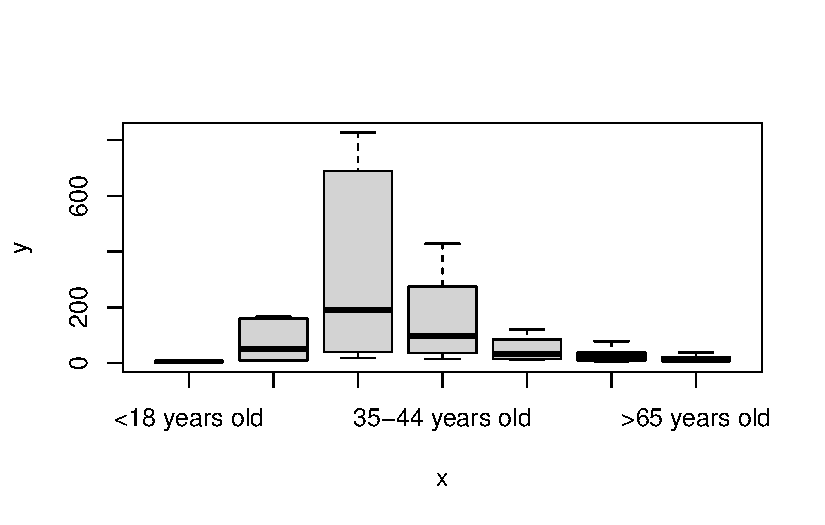
\includegraphics{Markdown_Section1.3_files/figure-pdf/unnamed-chunk-10-1.pdf}

}

\end{figure}

\begin{Shaded}
\begin{Highlighting}[]
\FunctionTok{plot}\NormalTok{(}\AttributeTok{x =}\NormalTok{ data3}\SpecialCharTok{$}\NormalTok{How.many.cups.of.coffee.do.you.typically.drink.per.day., }\AttributeTok{y =}\NormalTok{ data3}\SpecialCharTok{$}\NormalTok{Count)}
\end{Highlighting}
\end{Shaded}

\begin{figure}[H]

{\centering 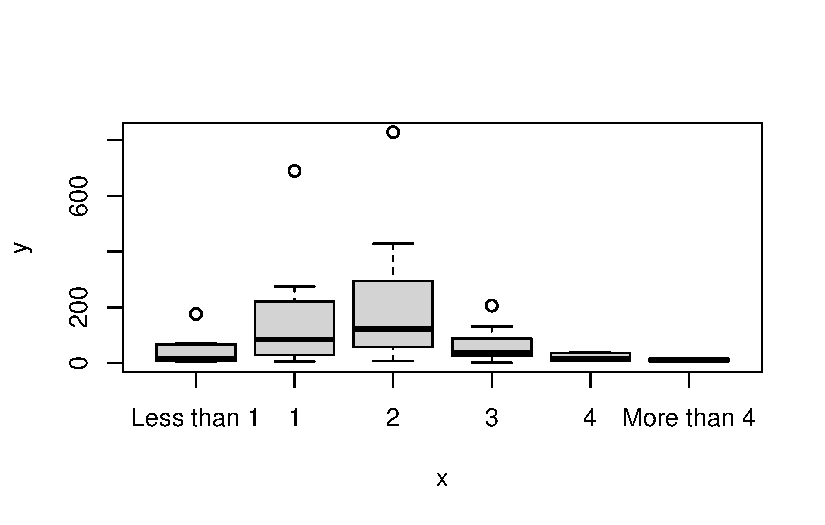
\includegraphics{Markdown_Section1.3_files/figure-pdf/unnamed-chunk-11-1.pdf}

}

\end{figure}

\hypertarget{save-the-data}{%
\chapter{4. Save the data}\label{save-the-data}}

\hypertarget{save-as-an-r-object}{%
\section{4.1 Save as an R object}\label{save-as-an-r-object}}

\begin{Shaded}
\begin{Highlighting}[]
\FunctionTok{save}\NormalTok{(data3, }\AttributeTok{file =} \StringTok{"data.Rdata"}\NormalTok{)}
\end{Highlighting}
\end{Shaded}

\hypertarget{save-as-a-csv-document}{%
\section{4.2 Save as a CSV document}\label{save-as-a-csv-document}}

\begin{Shaded}
\begin{Highlighting}[]
\FunctionTok{write.csv}\NormalTok{(data3, }\StringTok{"data3.csv"}\NormalTok{, }\AttributeTok{row.names =} \ConstantTok{FALSE}\NormalTok{)}
\end{Highlighting}
\end{Shaded}




\end{document}
